\hladd{
\section{Reuse and Warmstarting Optimizations}\label{sec-reuse-and-warmstarting}
With the experiment graph constructed and materialized, we can look for optimization opportunities for feature engineering and model training operations.
In this section, we propose two optimizations, namely, \textit{Reuse} and \textit{Warmstarting}.

Both reuse and warmstarting optimizations are part of the remote optimization step of Figure \ref{system-workflow}.
After computing workload execution subgraph (result of Step 2, Figure  \ref{system-workflow}), we query the experiment graph to look if any of the (non-computed) nodes in the workload execution subgraph exists and is materialized in the experiment graph.
Since during the materialization process (Section \ref{sec-materialization}) we have ensured the computation cost of a materialized vertex outweights its transfer cost, we can safely transfer the materialized vertex to the machine executing the workload.
Furthermore, We also look for warmstarting opportunities for any model training operations.
The result of Step 3 is another execution subgraph with (possibly) more edges pruned.
Finaly, we compute the execution plan using the the optimized execution subgraph (Step 4, Figure \ref{system-workflow}).

\subsection{Reuse}
The reuse process receives the workload execution subgraph as input and checks if there are matching vertices in the experiment graph.
%TODO define a theorem or somehow mention this rule
Based on the hashing procedure, we showed that two vertices belonging to two different graphs have the same hash if and only if they have the same execution subgraph.
Therefore, to find matching vertices in the workload execution subgraph, we query their id in the experiment graph.
However, in cases where the subgraph is very large and querying the experiment graph incurs a penalty, we must try to minimize the number of queries being made to the experiment graph.
In this section, we present three approaches for querying the experiment graph, namely, BottomUp reuse, TopDown reuse, and Hybrid reuse.

\textbf{BottomUp reuse.}
The process of BottomUp reuse is similar to how we construct the execution subgraph.
Algorithm \ref{algorithm-bottomup} shows the details of BottomUp reuse.
$v_t$ represent the vertex whose data is requested.
The BottomUp reuse utilizes the following early-stopping principle. 
If a vertex from the workload execution subgraph ($SG$) exist in the experiment graph ($EG$) and is materialized, then we can skip traversing its parents and return add the vertex to the set of returning materialized vertices.
Therefore, in Line 1, if $v_t$ is materialized, we return it as the result and in Lines 8-11, we only continue the search if the vertex ($v$) is not materialized ($is\_mat(EG, v)$ function returns true if $v$ is materialized in $EG$).
For any other vertex which is not materialized, we recursively examine its predecessors until we reach there are no more vertices left.

\begin{algorithm}[h]
\caption{BottomUp Reuse}\label{algorithm-bottomup}
\begin{algorithmic}[1]
\Require terminal vertex $v_t$, workload execution subgraph  $SG$, experiment graph $EG$ 
\Ensure set of materialized vertices $\mathcal{M}$ 
\If {$is\_mat(EG, v_t)$}
	\State return $\{v_t\}$
\EndIf
\State $Q \coloneqq  Queue(vt)$  
\State $\mathcal{M} \coloneqq \emptyset$
\While {$Q.not\_empty()$}
	\State $cur  \coloneqq  Q.pop()$
	\For {$v \in predecessors (SG, cur)$}
		\If {$is\_mat(EG, v)$}
			\State	$\mathcal{M}.append(v)$
		\Else
			\State $q.add(v)$
		\EndIf
	\EndFor
\EndWhile
\State return $\mathcal{M}$
\end{algorithmic}
\end{algorithm}
BottomUp approach performs well when the difference between the current workload graph and the ones that exist in the experiment graph are in vertices which are far from the root.
For example in Figure \ref{remote-optimization}, if vertex 7 or 6 were materialized, the BottomUp returns the result after one or two iterations, resulting in very few queries to the experiment graph.
On the other hand, the current workload differs with existing workloads in vertices close to the root, or in extreme scenarios, it has no similarity at all (a workload which works on a new root vertex), then BottomUp reuse has to traverse the graph until the root and queries the experiment graph for every vertex in the workload graph.

\textbf{TopDown reuse.}
Contrary to the BottomUp reuse, in TopDown reuse, we start traversing the workload execution subgraph, from its root vertices.

\begin{algorithm}[h]
\caption{TopDown Reuse}\label{algorithm-topdown}
\begin{algorithmic}[1]
\Require terminal vertex $v_t$, workload execution subgraph  $SG$, experiment graph $EG$ 
\Ensure set of materialized vertices $\mathcal{M}$ 
\State $R=roots(SG)$
\State $\mathcal{M} \coloneqq \emptyset$
\For {$r \in R$}
	\If {$r \notin EG$}
		\State continue \Comment{skip this iteration}
	\EndIf
	\State $Q \coloneqq  Queue(r)$  
	\If {$is\_mat(EG, r)$}
		 \State	 $\mathcal{M}.append(r)$
	\EndIf
		\While {$Q.not\_empty()$}
			\State $cur \coloneqq  Q.pop()$
			\For {$v \in children (SG, cur)$}
				\If {$is\_mat(EG, v)$}
					\State	$\mathcal{M}.append(v)$
				\EndIf
				\If {$v \in EG$} 
					\State $q.add(v)$
				\EndIf
			\EndFor
		\EndWhile
\EndFor
\State return $\mathcal{M}$
\end{algorithmic}
\end{algorithm}
Algorithm \ref{algorithm-topdown} shows the details of TopDown reuse method.
The TopDown reuse operates on the following early-stopping principle.
If a vertex from the workload execution subgraph ($SG$) does not exist in the experiment graph ($EG$), we terminate the traversal of its children.
This follows from the graph construction procedure, where each vertex is derived from its parents, as a result, it is impossible for a child vertex to exist in a graph where its parents do not.
Therefore, in Lines 4 and 14, we continue the traversal for a vertex if and only if the vertex is in the experiment graph.
Since a workload execution graph may have multiple root vertices, the TopDown reuse algorithm first finds all the root vertices (Line 1).
Then, for every root vertex, TopDown examines all of its children and add them to the set of materialized vertices if they are in the experiment graph and are materialized ($is\_mat$ returns true).
Unlike the BottomUp approach, when a node is materialized, we cannot stop the traversal, since a materialized vertex may also have materialized children.

TopDown can perform well in cases where BottomUp reuse performs poorly.
If the current workload operates on a completely new root (which never appeared in the experiment graph) or the workload contains early data exploration which never appeared in experiment graph, TopDown reuse will quickly stop the search process.
However, if the workload is very similar to previous workloads, the TopDown will perform many queries to the experiment graph.
An extreme example is when a workload is re-executed.
TopDown reuse will make one query for every vertex of the workload to the experiment graph before returning the materialized node.

\textbf{Hybrid reuse.}
Both BottomUp and TopDown reuse perform well in specific scenarios. 
However, neither of them can adapt to the different characteristics of a workload (e.g., how similar a work is to the previous workloads or how large the execution graph is).
We devise a dynamic reuse approach, called Hybrid reuse, which adapts to the current workload.
Algorithm \ref{algorithm-hybrid} shows the process of Hybrid reuse.
Hybrid reuse combines the two early-stopping principles utilized in TopDown and BottomUp reuse algorithms to prune the vertices without traversing them.
The BottomUp principle states that if a vertex is materialized in the experiment graph, we can skip traversing its predecessors.
The TopDown principle states that if a vertex is not in the experiment graph, then its children are also not in the experiment graph.
The Hyrbid reuse proceeds as follows.
It first traverse the vertices of the execution subgraph in reverse breadth-first-search order starting from the terminal vertex by calling the $R\_BFS(v, G, n\_visits)$, where $n\_visits$ indicate how many vertices should be traversed (Line 4).
However, unlike the BottomUp approach, the $R\_BFS$ procedure, only returns the vertex after $n\_visists$ vertices are visited and does not check if every vertex is in experiment graph or not.
Then, if the vertex returned is not in the experiment graph (Line 7), by following the TopDown principle, we can safely prune the bottom half of the graph and perform another reverse traversal.
If the vertex is materialized (Line 16), the algorithm utilizes the BottomUp principle and prunes the top half the graph.
Furthermore, when the vertex is materialized, the algorithm adds it to the list of the materialized vertices, and continues to traverse the graph in a forward breadth-first-search approach.
When the vertex is in the experiment graph but it is not materialized (Line 9), then there is no guarantee on if any part of the graph can be pruned.
However, we utilize the following heuristic to decide which part of the graph to prune.
We first compute the average value of the utility function for the parents and children of the vertex.
If the average value of the parents is greater than the children, then we prune the bottom half and continue to search using $R\_BFS$ in the top half of the graph.
Otherwise, we prune the top half and search in the bottom half using $F\_BFS$.
The intuition behind this heuristic is that if the parents of a node have a higher utility than its children, then there's a higher probability that there are vertices with higher potential and frequencies in the predecessors of the vertex which leads to higher utility value and increased chance of being materialized.

\begin{algorithm}[h]
\caption{Hybrid Reuse}\label{algorithm-hybrid}
\begin{algorithmic}[1]
\Require terminal vertex $v_t$, workload execution subgraph  $SG$, experiment graph $EG$ 
\Ensure set of materialized vertices $\mathcal{M}$ 
\State $N \coloneqq size(SG)$
\State $step \coloneqq 2$
\State $\mathcal{M} \coloneqq \emptyset$
\State $v \coloneqq R\_BFS(v_t, SG, N/step)$
\While {$step \leq log(N) $}
		\State $step = step \times 2$
		\If {$v \notin EG$}
				\State $v \coloneqq R\_BFS(v, SG, N/step)$
		\ElsIf {$v \in EG  \land \neg is\_mat(EG,v)$}
				\State $prev \coloneqq avg (\mathcal{U}(parents(EG, v))$
				\State $next \coloneqq avg (\mathcal{U}(children(EG, v))$
				\If{$prev \geq next $}
						 \State $v \coloneqq R\_BFS(v, SG, N/step)$
				\Else
					\State $v \coloneqq F\_BFS(v, SG, N/step)$
				\EndIf
		\ElsIf {$is\_math(EG, v)$}
				\State $\mathcal{M}.append(v)$
				\State $v \coloneqq F\_BFS(v, SG, N/step)$
		\EndIf
\EndWhile
\State return $\mathcal{M}$
\end{algorithmic}
\end{algorithm}
The advantage of the Hybrid reuse is that it requires at most $log(N)$ queries to the experiment graph, where $N$ is the size of the workload execution graph.
This is in contrast to the TopDown and BottomUp reuses, where in certain scenarios they may require $N$ queries to to experiment graph.
}

%We devise a strategy to detect overlapping operations in both the current workload and the experiment graph.
%If an operation already exists in the experiment graph, we directly access the resulting artifact in the experiment graph instead of executing the operation.
%Before executing a workload, we first transform it into its graph representation, which results in a directed graph, called $\mathcal{WG}$.
%Then, we traverse the experiment graph starting from the root node, using the edges of the workload graph.
%The result of the traversal is a subgraph of the experiment graph, which we refer to as $\mathcal{SG}$.
%The subgraph contains all the vertices and edges that exist in both the experiment graph and the workload graph.
%For every path in $\mathcal{SG}$ which originates at the root node, we return the furthest materialized vertex from the root node as the result and skip all the intermediate operations.
%
%To demonstrate with an example, let us assume a user has executed the code in Listing \ref{listing-experiment-graph} and Figure \ref{fig-experiment-graph}a shows the current experiment graph, where the set of materialized vertices is $\mathcal{MV} = \{v_0, v_2, v_3\}$.
%A new user submits the code in Listing \ref{listing-reuse}.
%Figure \ref{fig-reuse}a shows the workload graph ($\mathcal{WG}$) of the code in Listing \ref{listing-reuse}.
%As described in the Reuse procedure, we traverse the experiment graph, starting at $v_0$, with the edges of $\mathcal{WG}$ which results in the common subgraph, $\mathcal{SG}$, in Figure \ref{fig-reuse}b.
%In the subgraph $\mathcal{SG}$, the furthest vertices in each path originating at $v_0$ are $v_5$ and $v_3$.
%The Reuse procedure selects $v_2$ as the candidate since $v_5$ is not materialized.
%The Reuse procedure results in an optimized graph which skips operations p2 and p3 (Figure \ref{fig-reuse}c).
%% Tilmann: Can you elaborate the benefits? Also, what do the new reused nodes help? There does not seem to be a path to the final result from them. 
%
%\begin{lstlisting}[language=Python, firstnumber = 8,caption=New workload script (Imports are omitted),captionpos=b,label = {listing-reuse}]
%train = pd.read_csv('../input/train.csv') 
%selector =  SelectKBest(k=2)
%top_features = selector.fit_transform(train[['ts','u_id','price']], 
%				      train['y'])
%model = svm.SVC()
%model.fit(top_features, train['y'])
%\end{lstlisting}
%
%\begin{figure}
%\captionsetup[subfigure]{justification=centering}
%\begin{subfigure}[t]{0.33\linewidth}
%\centering
%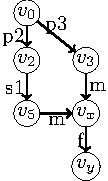
\includegraphics{../images/tikz-standalone/reuse-example-wg}
%\caption{Workload Graph ($\mathcal{WG}$)}
%\end{subfigure}%
%\begin{subfigure}[t]{0.33\linewidth}
%\centering
%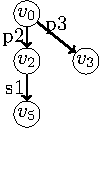
\includegraphics{../images/tikz-standalone/reuse-example-sg}
%\caption{Common Subgraph ($\mathcal{SG}$)}
%\end{subfigure}%
%\begin{subfigure}[t]{0.33\linewidth}
%\centering
%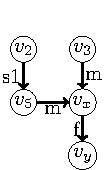
\includegraphics{../images/tikz-standalone/reuse-example-final}
%\caption{Optimized Graph}
%\end{subfigure}
%\begin{subfigure}[t]{\linewidth}
%\centering
%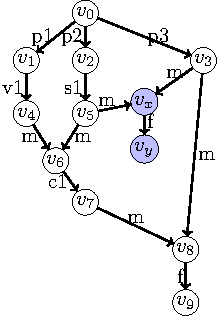
\includegraphics{../images/tikz-standalone/reuse-example-final-eg}
%\caption{Experiment graph after executing the workload (new nodes are highlighted)}
%\end{subfigure}
%\caption{Steps in the Reuse optimizations}
%\label{fig-reuse}
%\end{figure}
%
%\subsection{Warmstart Model Training Operations}
%Model training operations include extra hyperparameters that must be set before the training procedure begins.
%Two training operations on the same data artifact using the same training algorithm could potentially have very different results based on the values of the hyperparameters.
%Therefore, we cannot apply the Reuse optimization in cases the hyperparameters of model training operations are different.
%Instead, we apply the \textit{Warmstarting} optimization.
%We first need to describe the concept of model groups.
%For a vertex $v$, the model group $\mathcal{MG}_v$ refers to the set of all the machine learning models and their hyperparameters that are trained on $v$.
%If a workload contains the model training operation $e_{m}$ on the vertex $v_{m}$, before executing the workload, we proceed as follows.
%First, using the same traversal strategy as explained in the Reuse procedure, we look for $v_{m}$ in the experiment graph.
%If operation $e_{m}$ also exists in the experiment graph, then the Reuse procedure will return the resulting node as the result.
%However, if $e_{m}$ does not exist in the experiment graph, then we find the model group $\mathcal{MG}_{v_m}$.
%If $\mathcal{MG}_{v_m}$ is not empty, we warmstart the operation $e_{m}$ with the best performing model from the model group.
%% Tilmann: Does this always make sense? or do we get stuck in local minima this way?
%
%To demonstrate with an example, after executing both the code in Listings \ref{listing-experiment-graph} and \ref{listing-reuse}, a new users submits the same code as in Listing \ref{listing-reuse}, with a different model hyperparameters (Line 12) shown in Listing \ref{listing-warmstarting}.
%\begin{lstlisting}[language=Python, firstnumber=12, caption= Workload with different hyperparameters,captionpos=b,label = {listing-warmstarting}]
%model = svm.SVC(C=0.1)
%\end{lstlisting}
%Since both models (svm.SVC(C=0.1) and svm.SVC()) are trained on the same vertex ($v_x$ in Figure \ref{fig-reuse}), the Warmstarting procedure selects the existing model node ($v_y$ in Figure \ref{fig-reuse}) to warmstart the training process.
%
%Warmstarting can greatly reduce the total training time.
%However, the type of the machine learning model and the termination criteria play important roles in determining the effect of the warmstarting optimization.
%In the experiment section, we evaluate the effect of warmstarting on different types of models with different termination criteria.
%
%\subsubsection{Augmenting the experiment graph}
%When we utilize warmstarting, we extend the experiment graph with a merge operation which merges the dataset and the candidate model for warmstarting.
%The actual training operation is then applied to the merged node.
%As a result, we can keep track of the models that are utilized in warmstarting the training of other models which ensures reproducibility.
%
%Figure \ref{fig-warmstarting} shows the experiment graph after execution of the script from Listing \ref{listing-warmstarting}.
%The training operation, f1, is applied to the new vertex $v_n$, which is the result of merging the data artifact $v_x$ and the model $v_y$.
%The training operation f1 has a different hash from the existing operations since the hyperparameters are different.
%
%\begin{figure}[t]
%\centering
%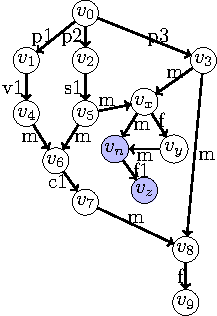
\includegraphics{../images/tikz-standalone/warmstarting-example-final-eg}
%\caption{Experiment graph after warmstarting} % Tilmann: Again, if v9 is the result, how does vx-vz contribute to this?
%\label{fig-warmstarting}
%\end{figure}

%For iterative training algorithms that are minimizing a loss function, there are two termination criteria, namely, the convergence tolerance and the number of iterations.
%
%\subsubsection{Convergence tolerance termination criteria}
%When the termination criteria of the model training operation in the workload is set to a specific convergence tolerance value, two scenarios may occur.
%In the first scenario, an existing trained model in the experiment graph has already reached the convergence tolerance value.
%In this scenario, we expect a large improvement in the training time as the training procedure in the workload will immediately converge.
%In the second scenario, no model in the experiment graph has reached the convergence tolerance value.
%In this case, we warmstart the model in the workload, to the model in the experiment graph with the highest attained quality.
%Therefore, we ensure the training procedure will converge faster.

%\subsubsection{Augmenting the experiment graph}
%Once the training procedure is finished, we augment the experiment graph with an edge and node representing the new model building operation and resulting model, respectively.
%\todo[inline]{We may need a special edge so that we know the training operation was not run from scratch and is the result of warmstarting.}

%\subsubsection{Partial Warmstarting Optimization For Model Training Operations}
%A common approach in machine learning workloads is to repeatedly select a different subset of features or create new features from the existing ones and train models on the new features.
%As a result, many model training operations operate on overlapping or different set of features.
%In the partial warmstarting optimization, we aim to improve the training time (and the quality) by warmstarting only the features that exist in the experiment database.

%\subsection{Reuse Optimization for Model Building Operations}
%Reuse for model building operations is more complicated.
%There are two types of reuse opportunities in the model building operations.
%
%\subsubsection{Exact Reuse}\label{sub-sub-exact-reuse}
%For non-user-defined aggregation operations, we follow the same procedure as the feature engineering processes.
%When the corresponding edge in the experiment graph has the same vertex and (aggregation) operation type, we reuse the result of the operation directly.
%We can also reuse the existing model training operation, if the input columns, algorithm, and all the hyper-parameters are the same.
%
%\subsubsection{Model parameter and hyper parameter warmstarting}\label{sub-sub-model-reuse}
%For the model training operations, 3 scenarios can occur.
%In the \textit{first scenario}, the training algorithm used for training the model has never been used before, therefore no meta-data about it exists in the experiment graph.
%In this scenario, no optimization is possible and the model training operation has to be executed completely.
%In the \textit{second scenario}, the training algorithm and the input columns to the model already exist in the experiment graph, but the specific hyperparameter setting does not.
%In this scenario, we can warmstart the model using the parameters from the corresponding node in the experiment graph.
%This reduces the training time as the model \hl{may} converge faster.
%\todo[inline]{This requires experiment and some math ?}
%In the \textit{third scenario}, the training algorithm and the hyperparameters are the same, but all the input columns do not exist in the corresponding node in the experiment graph.
%In this scenario, we provide partial warmstarting.
%In partial warmstarting, the model parameters corresponding to the columns of the input data that already exist in the experiment graph are warmstarted, and the rest of the parameters are randomly initialized.
%\todo[inline]{This requires experiment and some math ?}


%\subsection{Materialization of Grid Search}
%\todo[inline]{Incomplete}
%In order to analyze whether or not we should materialize parts of the grid search, we first have to unpack it, and compare it with other grid search.
%Then, similar to Section \ref{sub-sec-materialization-of-transformed-data}, we materialize the parts that are executed frequently.
%
%%\subsection{Guided Grid-Search}
%%\todo[inline]{just an idea}
%%By extracting correlation between different parameters and the model quality we can provided a guided grid search, where we can provide some estimate or show the effects of a hyperparameter range on the model quality